\documentclass[twoside]{book}

% Packages required by doxygen
\usepackage{fixltx2e}
\usepackage{calc}
\usepackage{doxygen}
\usepackage[export]{adjustbox} % also loads graphicx
\usepackage{graphicx}
\usepackage[utf8]{inputenc}
\usepackage{makeidx}
\usepackage{multicol}
\usepackage{multirow}
\PassOptionsToPackage{warn}{textcomp}
\usepackage{textcomp}
\usepackage[nointegrals]{wasysym}
\usepackage[table]{xcolor}

% Font selection
\usepackage[T1]{fontenc}
\usepackage[scaled=.90]{helvet}
\usepackage{courier}
\usepackage{amssymb}
\usepackage{sectsty}
\renewcommand{\familydefault}{\sfdefault}
\allsectionsfont{%
  \fontseries{bc}\selectfont%
  \color{darkgray}%
}
\renewcommand{\DoxyLabelFont}{%
  \fontseries{bc}\selectfont%
  \color{darkgray}%
}
\newcommand{\+}{\discretionary{\mbox{\scriptsize$\hookleftarrow$}}{}{}}

% Page & text layout
\usepackage{geometry}
\geometry{%
  a4paper,%
  top=2.5cm,%
  bottom=2.5cm,%
  left=2.5cm,%
  right=2.5cm%
}
\tolerance=750
\hfuzz=15pt
\hbadness=750
\setlength{\emergencystretch}{15pt}
\setlength{\parindent}{0cm}
\setlength{\parskip}{0.2cm}
\makeatletter
\renewcommand{\paragraph}{%
  \@startsection{paragraph}{4}{0ex}{-1.0ex}{1.0ex}{%
    \normalfont\normalsize\bfseries\SS@parafont%
  }%
}
\renewcommand{\subparagraph}{%
  \@startsection{subparagraph}{5}{0ex}{-1.0ex}{1.0ex}{%
    \normalfont\normalsize\bfseries\SS@subparafont%
  }%
}
\makeatother

% Headers & footers
\usepackage{fancyhdr}
\pagestyle{fancyplain}
\fancyhead[LE]{\fancyplain{}{\bfseries\thepage}}
\fancyhead[CE]{\fancyplain{}{}}
\fancyhead[RE]{\fancyplain{}{\bfseries\leftmark}}
\fancyhead[LO]{\fancyplain{}{\bfseries\rightmark}}
\fancyhead[CO]{\fancyplain{}{}}
\fancyhead[RO]{\fancyplain{}{\bfseries\thepage}}
\fancyfoot[LE]{\fancyplain{}{}}
\fancyfoot[CE]{\fancyplain{}{}}
\fancyfoot[RE]{\fancyplain{}{\bfseries\scriptsize Generated on Sat Dec 12 2015 19\+:04\+:50 for Doxygen by Doxygen }}
\fancyfoot[LO]{\fancyplain{}{\bfseries\scriptsize Generated on Sat Dec 12 2015 19\+:04\+:50 for Doxygen by Doxygen }}
\fancyfoot[CO]{\fancyplain{}{}}
\fancyfoot[RO]{\fancyplain{}{}}
\renewcommand{\footrulewidth}{0.4pt}
\renewcommand{\chaptermark}[1]{%
  \markboth{#1}{}%
}
\renewcommand{\sectionmark}[1]{%
  \markright{\thesection\ #1}%
}

% Indices & bibliography
\usepackage{natbib}
\usepackage[titles]{tocloft}
\setcounter{tocdepth}{3}
\setcounter{secnumdepth}{5}
\makeindex

% Hyperlinks (required, but should be loaded last)
\usepackage{ifpdf}
\ifpdf
  \usepackage[pdftex,pagebackref=true]{hyperref}
\else
  \usepackage[ps2pdf,pagebackref=true]{hyperref}
\fi
\hypersetup{%
  colorlinks=true,%
  linkcolor=blue,%
  citecolor=blue,%
  unicode%
}

% Custom commands
\newcommand{\clearemptydoublepage}{%
  \newpage{\pagestyle{empty}\cleardoublepage}%
}


%===== C O N T E N T S =====

\begin{document}

% Titlepage & ToC
\hypersetup{pageanchor=false,
             bookmarks=true,
             bookmarksnumbered=true,
             pdfencoding=unicode
            }
\pagenumbering{roman}
\begin{titlepage}
\vspace*{7cm}
\begin{center}%
{\Large Doxygen }\\
\vspace*{1cm}
{\large Generated by Doxygen 1.8.10}\\
\vspace*{0.5cm}
{\small Sat Dec 12 2015 19:04:50}\\
\end{center}
\end{titlepage}
\clearemptydoublepage
\tableofcontents
\clearemptydoublepage
\pagenumbering{arabic}
\hypersetup{pageanchor=true}

%--- Begin generated contents ---
\chapter{S\+E\+N\+G 330 Assignment 2}
\label{md__c_1__users__adewale__adekoya__documents__git_hub__a2__r_e_a_d_m_e}
\hypertarget{md__c_1__users__adewale__adekoya__documents__git_hub__a2__r_e_a_d_m_e}{}
Adewale Adekoya E

I\+N\+S\+T\+R\+U\+C\+T\+O\+R \+: G\+E\+O\+R\+G\+E T\+Z\+A\+N\+E\+T\+A\+K\+I\+S 
\chapter{Hierarchical Index}
\section{Class Hierarchy}
This inheritance list is sorted roughly, but not completely, alphabetically\+:\begin{DoxyCompactList}
\item \contentsline{section}{Actor}{\pageref{class_actor}}{}
\begin{DoxyCompactList}
\item \contentsline{section}{Character}{\pageref{class_character}}{}
\end{DoxyCompactList}
\item Message\begin{DoxyCompactList}
\item \contentsline{section}{proto\+:\+:Character}{\pageref{classproto_1_1_character}}{}
\end{DoxyCompactList}
\item \contentsline{section}{Skill}{\pageref{struct_skill}}{}
\item \contentsline{section}{Skill\+Type}{\pageref{class_skill_type}}{}
\item \contentsline{section}{proto\+:\+:Static\+Descriptor\+Initializer\+\_\+\+Character\+\_\+2eproto}{\pageref{structproto_1_1_static_descriptor_initializer___character__2eproto}}{}
\item \contentsline{section}{Weapon}{\pageref{struct_weapon}}{}
\end{DoxyCompactList}

\chapter{Class Index}
\section{Class List}
Here are the classes, structs, unions and interfaces with brief descriptions\+:\begin{DoxyCompactList}
\item\contentsline{section}{\hyperlink{class_actor}{Actor} }{\pageref{class_actor}}{}
\item\contentsline{section}{\hyperlink{class_character}{Character} }{\pageref{class_character}}{}
\item\contentsline{section}{\hyperlink{classproto_1_1_character}{proto\+::\+Character} }{\pageref{classproto_1_1_character}}{}
\item\contentsline{section}{\hyperlink{struct_skill}{Skill} }{\pageref{struct_skill}}{}
\item\contentsline{section}{\hyperlink{class_skill_type}{Skill\+Type} }{\pageref{class_skill_type}}{}
\item\contentsline{section}{\hyperlink{structproto_1_1_static_descriptor_initializer___character__2eproto}{proto\+::\+Static\+Descriptor\+Initializer\+\_\+\+Character\+\_\+2eproto} }{\pageref{structproto_1_1_static_descriptor_initializer___character__2eproto}}{}
\item\contentsline{section}{\hyperlink{struct_weapon}{Weapon} }{\pageref{struct_weapon}}{}
\end{DoxyCompactList}

\chapter{Class Documentation}
\hypertarget{class_actor}{}\section{Actor Class Reference}
\label{class_actor}\index{Actor@{Actor}}
Inheritance diagram for Actor\+:\begin{figure}[H]
\begin{center}
\leavevmode
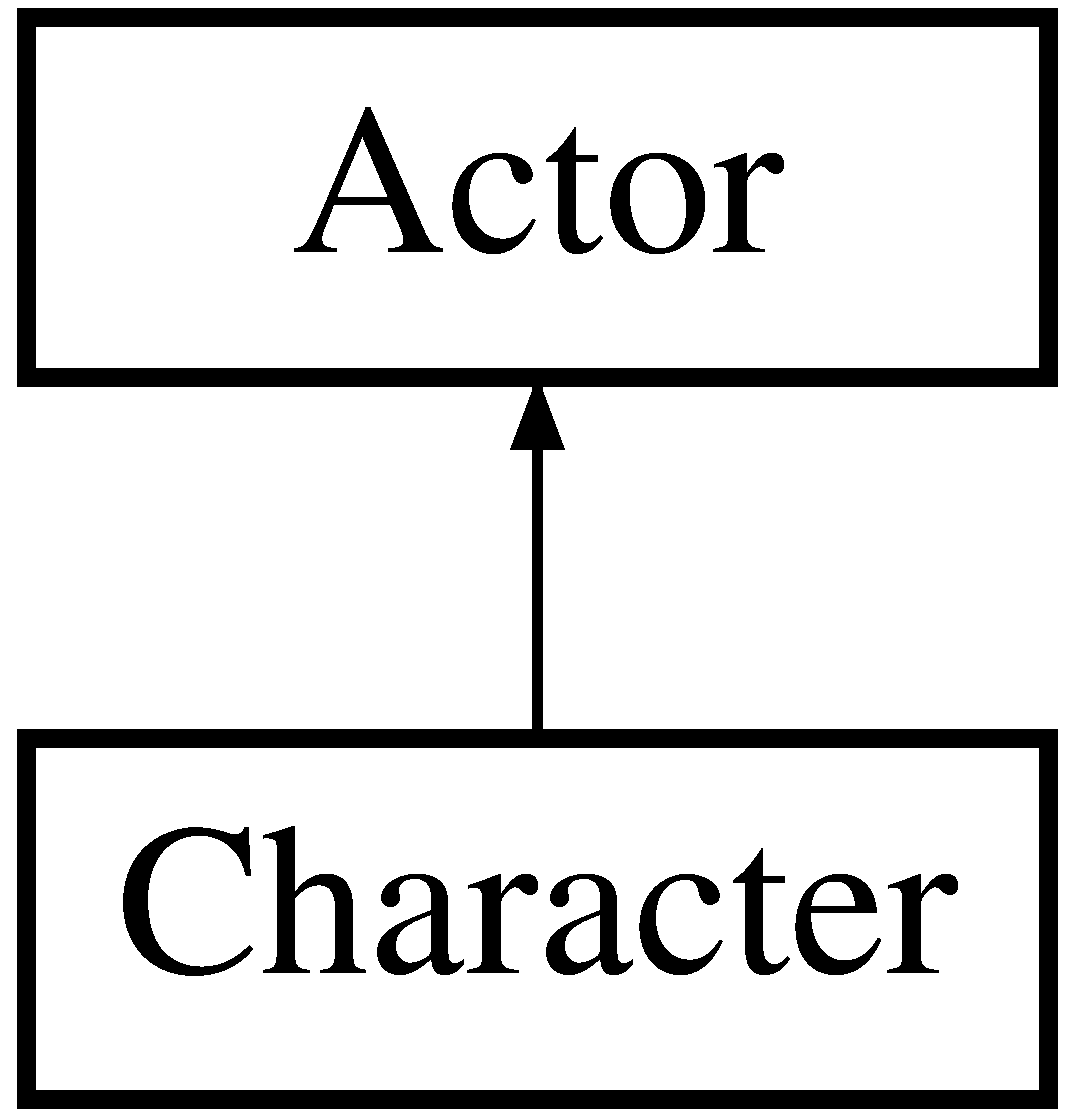
\includegraphics[height=2.000000cm]{class_actor}
\end{center}
\end{figure}
\subsection*{Public Member Functions}
\begin{DoxyCompactItemize}
\item 
virtual void \hyperlink{class_actor_ad5c98db519558b3b22c03acec73b8869}{Draw} (sf\+::\+Render\+Window \&window)=0
\item 
virtual void \hyperlink{class_actor_a41012afefccde8234e574b03d9fdbc08}{Set\+Position} (const float \&x\+Position, const float \&y\+Position)
\item 
sf\+::\+Vector2f \hyperlink{class_actor_a2f63a8afe2d15b4ba695b2d4e4c8597e}{Get\+Dimensions} () const 
\end{DoxyCompactItemize}
\subsection*{Protected Attributes}
\begin{DoxyCompactItemize}
\item 
sf\+::\+Vector2f \hyperlink{class_actor_acfabf742ec617868223278c3b8f91336}{\+\_\+dimensions}
\item 
sf\+::\+Vector2f \hyperlink{class_actor_ad3760883a99be5b4aaa2635ca761c29b}{\+\_\+position}
\end{DoxyCompactItemize}


\subsection{Member Function Documentation}
\hypertarget{class_actor_ad5c98db519558b3b22c03acec73b8869}{}\index{Actor@{Actor}!Draw@{Draw}}
\index{Draw@{Draw}!Actor@{Actor}}
\subsubsection[{Draw(sf\+::\+Render\+Window \&window)=0}]{\setlength{\rightskip}{0pt plus 5cm}virtual void Actor\+::\+Draw (
\begin{DoxyParamCaption}
\item[{sf\+::\+Render\+Window \&}]{window}
\end{DoxyParamCaption}
)\hspace{0.3cm}{\ttfamily [pure virtual]}}\label{class_actor_ad5c98db519558b3b22c03acec73b8869}
Draws a new frame given an sfml window object.


\begin{DoxyParams}{Parameters}
{\em window} & -\/ a reference to a window that serves as a target for 2\+D drawing. \\
\hline
\end{DoxyParams}


Implemented in \hyperlink{class_character_a5816034e10d2ef4610719ad0a68e7314}{Character}.

\hypertarget{class_actor_a2f63a8afe2d15b4ba695b2d4e4c8597e}{}\index{Actor@{Actor}!Get\+Dimensions@{Get\+Dimensions}}
\index{Get\+Dimensions@{Get\+Dimensions}!Actor@{Actor}}
\subsubsection[{Get\+Dimensions() const }]{\setlength{\rightskip}{0pt plus 5cm}sf\+::\+Vector2f Actor\+::\+Get\+Dimensions (
\begin{DoxyParamCaption}
{}
\end{DoxyParamCaption}
) const\hspace{0.3cm}{\ttfamily [inline]}}\label{class_actor_a2f63a8afe2d15b4ba695b2d4e4c8597e}
Returns the actor\textquotesingle{}s dimensions.

\begin{DoxyReturn}{Returns}
a 2\+D S\+F\+M\+L vector describing the actor\textquotesingle{}s dimensions 
\end{DoxyReturn}
\hypertarget{class_actor_a41012afefccde8234e574b03d9fdbc08}{}\index{Actor@{Actor}!Set\+Position@{Set\+Position}}
\index{Set\+Position@{Set\+Position}!Actor@{Actor}}
\subsubsection[{Set\+Position(const float \&x\+Position, const float \&y\+Position)}]{\setlength{\rightskip}{0pt plus 5cm}virtual void Actor\+::\+Set\+Position (
\begin{DoxyParamCaption}
\item[{const float \&}]{x\+Position, }
\item[{const float \&}]{y\+Position}
\end{DoxyParamCaption}
)\hspace{0.3cm}{\ttfamily [inline]}, {\ttfamily [virtual]}}\label{class_actor_a41012afefccde8234e574b03d9fdbc08}
Sets the actor\textquotesingle{}s position in the window.


\begin{DoxyParams}{Parameters}
{\em x\+Position} & -\/ a constant reference to a floating point value which represents the x axis \\
\hline
{\em y\+Position} & -\/ a constant reference to a floating point value which represents the y axis \\
\hline
\end{DoxyParams}


Reimplemented in \hyperlink{class_character_a6fd2cc7114d91771abc82f223bde585b}{Character}.



\subsection{Member Data Documentation}
\hypertarget{class_actor_acfabf742ec617868223278c3b8f91336}{}\index{Actor@{Actor}!\+\_\+dimensions@{\+\_\+dimensions}}
\index{\+\_\+dimensions@{\+\_\+dimensions}!Actor@{Actor}}
\subsubsection[{\+\_\+dimensions}]{\setlength{\rightskip}{0pt plus 5cm}sf\+::\+Vector2f Actor\+::\+\_\+dimensions\hspace{0.3cm}{\ttfamily [protected]}}\label{class_actor_acfabf742ec617868223278c3b8f91336}
A 2\+D vector containing the dimensions of the actor. \hypertarget{class_actor_ad3760883a99be5b4aaa2635ca761c29b}{}\index{Actor@{Actor}!\+\_\+position@{\+\_\+position}}
\index{\+\_\+position@{\+\_\+position}!Actor@{Actor}}
\subsubsection[{\+\_\+position}]{\setlength{\rightskip}{0pt plus 5cm}sf\+::\+Vector2f Actor\+::\+\_\+position\hspace{0.3cm}{\ttfamily [protected]}}\label{class_actor_ad3760883a99be5b4aaa2635ca761c29b}
A 2\+D vector containing the position of the actor. 

The documentation for this class was generated from the following file\+:\begin{DoxyCompactItemize}
\item 
C\+:/\+Users/\+Adewale Adekoya/\+Documents/\+Git\+Hub/\+A2/Actor.\+h\end{DoxyCompactItemize}

\hypertarget{class_character}{}\section{Character Class Reference}
\label{class_character}\index{Character@{Character}}


{\ttfamily \#include $<$Character.\+h$>$}

Inheritance diagram for Character\+:\begin{figure}[H]
\begin{center}
\leavevmode
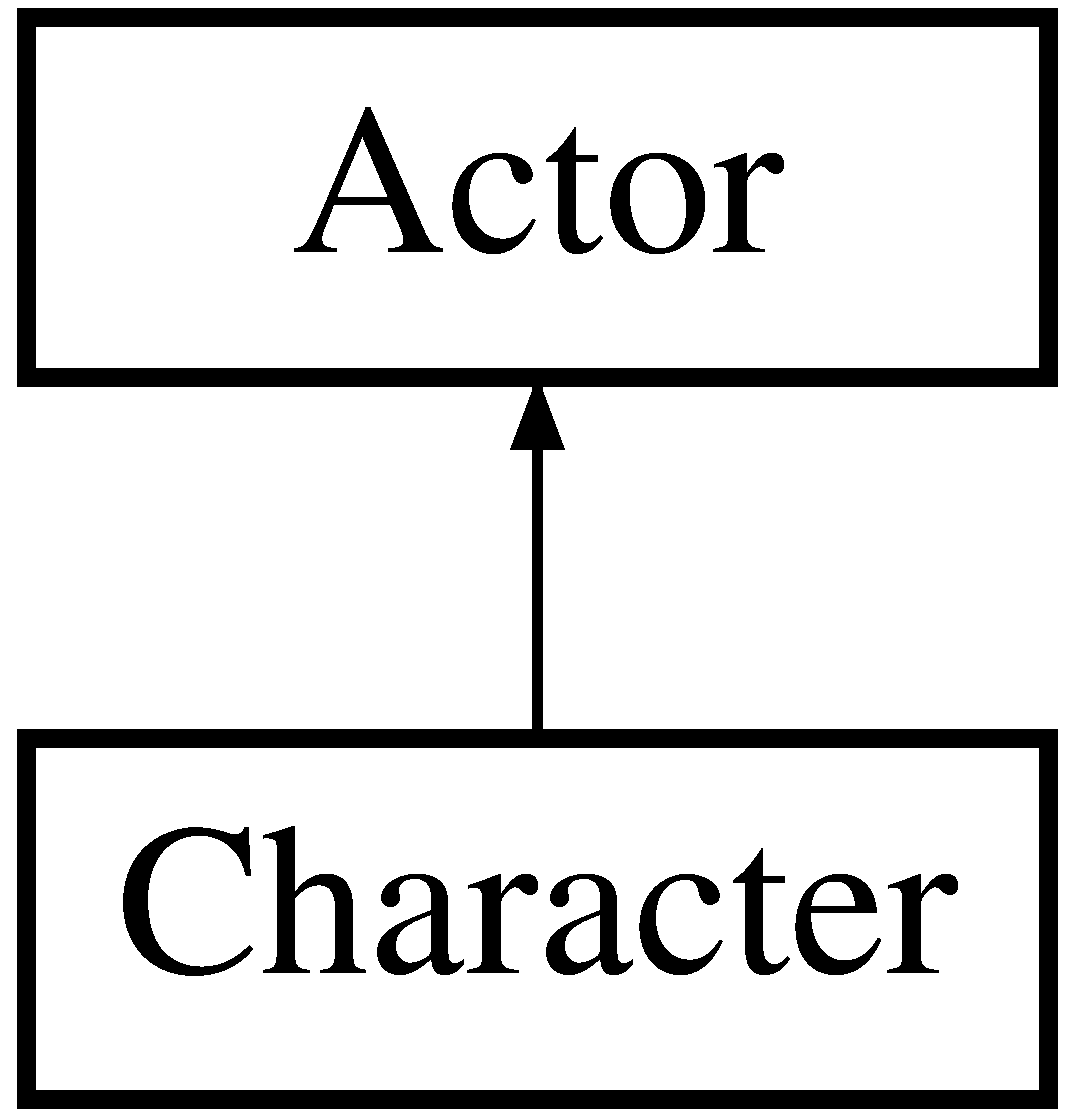
\includegraphics[height=2.000000cm]{class_character}
\end{center}
\end{figure}
\subsection*{Public Member Functions}
\begin{DoxyCompactItemize}
\item 
\hyperlink{class_character_a4c236e411ce0bf61200c4d88e36debc5}{Character} (const \hyperlink{class_character}{Character} \&a)
\item 
\hyperlink{class_character_a9e9be564d05ded80962b2045aa70b3fc}{$\sim$\+Character} ()
\item 
std\+::string \hyperlink{class_character_a8a39d33ea6e7520b61f3c083785d6035}{Get\+Name} () const 
\item 
unsigned \hyperlink{class_character_ad44a3a5644c62a4ae4feec398c77a137}{Get\+Level} () const 
\item 
unsigned \hyperlink{class_character_a6453138461bf9f62bdaeb07de9dacf8b}{Get\+Health} () const 
\item 
Character\+Class \hyperlink{class_character_abf7b793cda16b5924903d434de9e40a9}{Get\+Class} () const 
\item 
unsigned \hyperlink{class_character_a665088d6f0172b71cec106b68360a56a}{Get\+Wins} () const 
\item 
unsigned \hyperlink{class_character_a2a2b3a0964d0bffd300d7fcc34965376}{Get\+Losses} () const 
\item 
void \hyperlink{class_character_a6b5c00e13c98e143b10e7423fde49384}{Incrementwins} ()
\item 
void \hyperlink{class_character_ae810911be58f43ca4189b563383f1a49}{Increment\+Losses} ()
\item 
unsigned \hyperlink{class_character_a2bfad59dee714068f3f196fde4f47221}{Get\+Xp} () const 
\item 
void \hyperlink{class_character_a34ef80145d40f2d859b98398ec1be189}{Update\+Level} ()
\item 
bool \hyperlink{class_character_a73300e57fa813cf193c8f858ca081fd6}{Get\+Level\+Up} () const 
\item 
void \hyperlink{class_character_a08899a991714b1b880962064557e34bc}{Take\+Damage} (const unsigned \&damage)
\item 
void \hyperlink{class_character_a5816034e10d2ef4610719ad0a68e7314}{Draw} (sf\+::\+Render\+Window \&window) override
\item 
void \hyperlink{class_character_a6fd2cc7114d91771abc82f223bde585b}{Set\+Position} (const float \&x\+Position, const float \&y\+Position) override
\end{DoxyCompactItemize}
\subsection*{Protected Attributes}
\begin{DoxyCompactItemize}
\item 
const std\+::string \hyperlink{class_character_aa86be1de1ef615913a552b2134fbb966}{\+\_\+name}
\item 
unsigned \hyperlink{class_character_ab76c68c70f6b8a7dd0d70291cfaeacaf}{\+\_\+level}
\item 
unsigned \hyperlink{class_character_a143e6724430834bf37d93efe4c8d4f98}{\+\_\+health}
\item 
unsigned \hyperlink{class_character_a68d70b5ab4f09cd2a74524fc3d162d3d}{\+\_\+num\+Wins}
\item 
unsigned \hyperlink{class_character_a0f2af69ac7a82ebff650b1a430bb4331}{\+\_\+num\+Losses}
\item 
unsigned \hyperlink{class_character_a1155ad0a6f019df868ce25fb18767c3d}{\+\_\+xp}
\item 
bool \hyperlink{class_character_a7d661e1d0a7631b0c5a2a06ef0165090}{\+\_\+levelup}
\item 
sf\+::\+Sprite \hyperlink{class_character_ab3b89d967b817bc3e199ed70f6b6277a}{\+\_\+sprite}
\item 
sf\+::\+Image \hyperlink{class_character_a1a8bdd55f5f5ec76eabc83c28f0207e4}{\+\_\+sprite\+\_\+image}
\item 
sf\+::\+Texture \hyperlink{class_character_aced7e12300ddeaee16c95850e028b10f}{\+\_\+sprite\+\_\+texture}
\item 
const Character\+Class \hyperlink{class_character_a1027f1708720c0f9bbf0da8c4ae10d97}{\+\_\+class}
\end{DoxyCompactItemize}


\subsection{Detailed Description}
A \hyperlink{class_character}{Character} extends \hyperlink{class_actor}{Actor}. It contains character attributes that are used by human and A\+I players. 

\subsection{Constructor \& Destructor Documentation}
\hypertarget{class_character_a4c236e411ce0bf61200c4d88e36debc5}{}\index{Character@{Character}!Character@{Character}}
\index{Character@{Character}!Character@{Character}}
\subsubsection[{Character(const Character \&a)}]{\setlength{\rightskip}{0pt plus 5cm}Character\+::\+Character (
\begin{DoxyParamCaption}
\item[{const {\bf Character} \&}]{a}
\end{DoxyParamCaption}
)}\label{class_character_a4c236e411ce0bf61200c4d88e36debc5}
Copy constructor for the \hyperlink{class_character}{Character} class \hypertarget{class_character_a9e9be564d05ded80962b2045aa70b3fc}{}\index{Character@{Character}!````~Character@{$\sim$\+Character}}
\index{````~Character@{$\sim$\+Character}!Character@{Character}}
\subsubsection[{$\sim$\+Character()}]{\setlength{\rightskip}{0pt plus 5cm}Character\+::$\sim$\+Character (
\begin{DoxyParamCaption}
{}
\end{DoxyParamCaption}
)\hspace{0.3cm}{\ttfamily [inline]}}\label{class_character_a9e9be564d05ded80962b2045aa70b3fc}
\hyperlink{class_character}{Character} class deconstructor. 

\subsection{Member Function Documentation}
\hypertarget{class_character_a5816034e10d2ef4610719ad0a68e7314}{}\index{Character@{Character}!Draw@{Draw}}
\index{Draw@{Draw}!Character@{Character}}
\subsubsection[{Draw(sf\+::\+Render\+Window \&window) override}]{\setlength{\rightskip}{0pt plus 5cm}void Character\+::\+Draw (
\begin{DoxyParamCaption}
\item[{sf\+::\+Render\+Window \&}]{window}
\end{DoxyParamCaption}
)\hspace{0.3cm}{\ttfamily [override]}, {\ttfamily [virtual]}}\label{class_character_a5816034e10d2ef4610719ad0a68e7314}
\hyperlink{class_actor}{Actor} Interface\+: draws the \hyperlink{class_character}{Character}.

The Draw implementation for the \hyperlink{class_character}{Character} class which draws the \hyperlink{class_character}{Character}\textquotesingle{}s sprite. 

Implements \hyperlink{class_actor_ad5c98db519558b3b22c03acec73b8869}{Actor}.

\hypertarget{class_character_abf7b793cda16b5924903d434de9e40a9}{}\index{Character@{Character}!Get\+Class@{Get\+Class}}
\index{Get\+Class@{Get\+Class}!Character@{Character}}
\subsubsection[{Get\+Class() const }]{\setlength{\rightskip}{0pt plus 5cm}Character\+Class Character\+::\+Get\+Class (
\begin{DoxyParamCaption}
{}
\end{DoxyParamCaption}
) const}\label{class_character_abf7b793cda16b5924903d434de9e40a9}
Returns the \hyperlink{class_character}{Character}\textquotesingle{}s class object.

\begin{DoxyReturn}{Returns}
the Character\+Class specification of the \hyperlink{class_character}{Character}.
\end{DoxyReturn}
Returns the \hyperlink{class_character}{Character}\textquotesingle{}s class \hypertarget{class_character_a6453138461bf9f62bdaeb07de9dacf8b}{}\index{Character@{Character}!Get\+Health@{Get\+Health}}
\index{Get\+Health@{Get\+Health}!Character@{Character}}
\subsubsection[{Get\+Health() const }]{\setlength{\rightskip}{0pt plus 5cm}unsigned Character\+::\+Get\+Health (
\begin{DoxyParamCaption}
{}
\end{DoxyParamCaption}
) const}\label{class_character_a6453138461bf9f62bdaeb07de9dacf8b}
Returns the \hyperlink{class_character}{Character}\textquotesingle{}s health.

\begin{DoxyReturn}{Returns}
the health of the \hyperlink{class_character}{Character}, represented as an unsigned number
\end{DoxyReturn}
Returns the \hyperlink{class_character}{Character}\textquotesingle{}s health \hypertarget{class_character_ad44a3a5644c62a4ae4feec398c77a137}{}\index{Character@{Character}!Get\+Level@{Get\+Level}}
\index{Get\+Level@{Get\+Level}!Character@{Character}}
\subsubsection[{Get\+Level() const }]{\setlength{\rightskip}{0pt plus 5cm}unsigned Character\+::\+Get\+Level (
\begin{DoxyParamCaption}
{}
\end{DoxyParamCaption}
) const}\label{class_character_ad44a3a5644c62a4ae4feec398c77a137}
Returns the \hyperlink{class_character}{Character}\textquotesingle{}s level.

\begin{DoxyReturn}{Returns}
the level of the \hyperlink{class_character}{Character}, represented as an unsigned number
\end{DoxyReturn}
Returns the \hyperlink{class_character}{Character}\textquotesingle{}s level \hypertarget{class_character_a73300e57fa813cf193c8f858ca081fd6}{}\index{Character@{Character}!Get\+Level\+Up@{Get\+Level\+Up}}
\index{Get\+Level\+Up@{Get\+Level\+Up}!Character@{Character}}
\subsubsection[{Get\+Level\+Up() const }]{\setlength{\rightskip}{0pt plus 5cm}bool Character\+::\+Get\+Level\+Up (
\begin{DoxyParamCaption}
{}
\end{DoxyParamCaption}
) const}\label{class_character_a73300e57fa813cf193c8f858ca081fd6}
Determines if the level needs to be updated.

\begin{DoxyReturn}{Returns}
a boolean value indicating whether the \hyperlink{class_character}{Character} can level up 
\end{DoxyReturn}
\hypertarget{class_character_a2a2b3a0964d0bffd300d7fcc34965376}{}\index{Character@{Character}!Get\+Losses@{Get\+Losses}}
\index{Get\+Losses@{Get\+Losses}!Character@{Character}}
\subsubsection[{Get\+Losses() const }]{\setlength{\rightskip}{0pt plus 5cm}unsigned Character\+::\+Get\+Losses (
\begin{DoxyParamCaption}
{}
\end{DoxyParamCaption}
) const}\label{class_character_a2a2b3a0964d0bffd300d7fcc34965376}
Returns the \hyperlink{class_character}{Character}\textquotesingle{}s number of Losses.

\begin{DoxyReturn}{Returns}
the number of times the \hyperlink{class_character}{Character} has lost
\end{DoxyReturn}
Returns the \hyperlink{class_character}{Character}\textquotesingle{}s number of losses \hypertarget{class_character_a8a39d33ea6e7520b61f3c083785d6035}{}\index{Character@{Character}!Get\+Name@{Get\+Name}}
\index{Get\+Name@{Get\+Name}!Character@{Character}}
\subsubsection[{Get\+Name() const }]{\setlength{\rightskip}{0pt plus 5cm}std\+::string Character\+::\+Get\+Name (
\begin{DoxyParamCaption}
{}
\end{DoxyParamCaption}
) const}\label{class_character_a8a39d33ea6e7520b61f3c083785d6035}
Returns the \hyperlink{class_character}{Character}\textquotesingle{}s name.

\begin{DoxyReturn}{Returns}
the name of the \hyperlink{class_character}{Character}
\end{DoxyReturn}
Returns the \hyperlink{class_character}{Character}\textquotesingle{}s name \hypertarget{class_character_a665088d6f0172b71cec106b68360a56a}{}\index{Character@{Character}!Get\+Wins@{Get\+Wins}}
\index{Get\+Wins@{Get\+Wins}!Character@{Character}}
\subsubsection[{Get\+Wins() const }]{\setlength{\rightskip}{0pt plus 5cm}unsigned Character\+::\+Get\+Wins (
\begin{DoxyParamCaption}
{}
\end{DoxyParamCaption}
) const}\label{class_character_a665088d6f0172b71cec106b68360a56a}
Returns the \hyperlink{class_character}{Character}\textquotesingle{}s number of wins.

\begin{DoxyReturn}{Returns}
the number of times the \hyperlink{class_character}{Character} has won
\end{DoxyReturn}
Returns the \hyperlink{class_character}{Character}\textquotesingle{}s number of wins \hypertarget{class_character_a2bfad59dee714068f3f196fde4f47221}{}\index{Character@{Character}!Get\+Xp@{Get\+Xp}}
\index{Get\+Xp@{Get\+Xp}!Character@{Character}}
\subsubsection[{Get\+Xp() const }]{\setlength{\rightskip}{0pt plus 5cm}unsigned Character\+::\+Get\+Xp (
\begin{DoxyParamCaption}
{}
\end{DoxyParamCaption}
) const}\label{class_character_a2bfad59dee714068f3f196fde4f47221}
Returns the \hyperlink{class_character}{Character}\textquotesingle{}s current X\+P.

\begin{DoxyReturn}{Returns}
the current X\+P (experience) that the \hyperlink{class_character}{Character} has as an unsigned number
\end{DoxyReturn}
Returns the \hyperlink{class_character}{Character}\textquotesingle{}s current X\+P. \hypertarget{class_character_ae810911be58f43ca4189b563383f1a49}{}\index{Character@{Character}!Increment\+Losses@{Increment\+Losses}}
\index{Increment\+Losses@{Increment\+Losses}!Character@{Character}}
\subsubsection[{Increment\+Losses()}]{\setlength{\rightskip}{0pt plus 5cm}void Character\+::\+Increment\+Losses (
\begin{DoxyParamCaption}
{}
\end{DoxyParamCaption}
)}\label{class_character_ae810911be58f43ca4189b563383f1a49}
Updates the number of losses. This method increments the number of losses for the \hyperlink{class_character}{Character}.

This method also decreases X\+P by 25 or sets it to zero. \hypertarget{class_character_a6b5c00e13c98e143b10e7423fde49384}{}\index{Character@{Character}!Incrementwins@{Incrementwins}}
\index{Incrementwins@{Incrementwins}!Character@{Character}}
\subsubsection[{Incrementwins()}]{\setlength{\rightskip}{0pt plus 5cm}void Character\+::\+Incrementwins (
\begin{DoxyParamCaption}
{}
\end{DoxyParamCaption}
)}\label{class_character_a6b5c00e13c98e143b10e7423fde49384}
Updates the number of wins. This method increments the number of wins for the \hyperlink{class_character}{Character}.

This method also increases the X\+P by 50 and updates the \hyperlink{class_character}{Character}\textquotesingle{}s level. \hypertarget{class_character_a6fd2cc7114d91771abc82f223bde585b}{}\index{Character@{Character}!Set\+Position@{Set\+Position}}
\index{Set\+Position@{Set\+Position}!Character@{Character}}
\subsubsection[{Set\+Position(const float \&x\+Position, const float \&y\+Position) override}]{\setlength{\rightskip}{0pt plus 5cm}void Character\+::\+Set\+Position (
\begin{DoxyParamCaption}
\item[{const float \&}]{x\+Position, }
\item[{const float \&}]{y\+Position}
\end{DoxyParamCaption}
)\hspace{0.3cm}{\ttfamily [override]}, {\ttfamily [virtual]}}\label{class_character_a6fd2cc7114d91771abc82f223bde585b}
\hyperlink{class_actor}{Actor} Interface\+: specifies the position of the \hyperlink{class_character}{Character}.

Position override that also sets the sprite position. 

Reimplemented from \hyperlink{class_actor_a41012afefccde8234e574b03d9fdbc08}{Actor}.

\hypertarget{class_character_a08899a991714b1b880962064557e34bc}{}\index{Character@{Character}!Take\+Damage@{Take\+Damage}}
\index{Take\+Damage@{Take\+Damage}!Character@{Character}}
\subsubsection[{Take\+Damage(const unsigned \&damage)}]{\setlength{\rightskip}{0pt plus 5cm}void Character\+::\+Take\+Damage (
\begin{DoxyParamCaption}
\item[{const unsigned \&}]{damage}
\end{DoxyParamCaption}
)}\label{class_character_a08899a991714b1b880962064557e34bc}
Deals damage taken while playing a round.

Deals damage taken while in match. \hypertarget{class_character_a34ef80145d40f2d859b98398ec1be189}{}\index{Character@{Character}!Update\+Level@{Update\+Level}}
\index{Update\+Level@{Update\+Level}!Character@{Character}}
\subsubsection[{Update\+Level()}]{\setlength{\rightskip}{0pt plus 5cm}void Character\+::\+Update\+Level (
\begin{DoxyParamCaption}
{}
\end{DoxyParamCaption}
)}\label{class_character_a34ef80145d40f2d859b98398ec1be189}
Updates the level.

Updates the current level of player. 

\subsection{Member Data Documentation}
\hypertarget{class_character_a1027f1708720c0f9bbf0da8c4ae10d97}{}\index{Character@{Character}!\+\_\+class@{\+\_\+class}}
\index{\+\_\+class@{\+\_\+class}!Character@{Character}}
\subsubsection[{\+\_\+class}]{\setlength{\rightskip}{0pt plus 5cm}const Character\+Class Character\+::\+\_\+class\hspace{0.3cm}{\ttfamily [protected]}}\label{class_character_a1027f1708720c0f9bbf0da8c4ae10d97}
The \hyperlink{class_character}{Character}\textquotesingle{}s class. \hypertarget{class_character_a143e6724430834bf37d93efe4c8d4f98}{}\index{Character@{Character}!\+\_\+health@{\+\_\+health}}
\index{\+\_\+health@{\+\_\+health}!Character@{Character}}
\subsubsection[{\+\_\+health}]{\setlength{\rightskip}{0pt plus 5cm}unsigned Character\+::\+\_\+health\hspace{0.3cm}{\ttfamily [protected]}}\label{class_character_a143e6724430834bf37d93efe4c8d4f98}
The amount of health that the \hyperlink{class_character}{Character} has. \hypertarget{class_character_ab76c68c70f6b8a7dd0d70291cfaeacaf}{}\index{Character@{Character}!\+\_\+level@{\+\_\+level}}
\index{\+\_\+level@{\+\_\+level}!Character@{Character}}
\subsubsection[{\+\_\+level}]{\setlength{\rightskip}{0pt plus 5cm}unsigned Character\+::\+\_\+level\hspace{0.3cm}{\ttfamily [protected]}}\label{class_character_ab76c68c70f6b8a7dd0d70291cfaeacaf}
The \hyperlink{class_character}{Character}\textquotesingle{}s current level. \hypertarget{class_character_a7d661e1d0a7631b0c5a2a06ef0165090}{}\index{Character@{Character}!\+\_\+levelup@{\+\_\+levelup}}
\index{\+\_\+levelup@{\+\_\+levelup}!Character@{Character}}
\subsubsection[{\+\_\+levelup}]{\setlength{\rightskip}{0pt plus 5cm}bool Character\+::\+\_\+levelup\hspace{0.3cm}{\ttfamily [protected]}}\label{class_character_a7d661e1d0a7631b0c5a2a06ef0165090}
Contains whether the \hyperlink{class_character}{Character} has leveled up. \hypertarget{class_character_aa86be1de1ef615913a552b2134fbb966}{}\index{Character@{Character}!\+\_\+name@{\+\_\+name}}
\index{\+\_\+name@{\+\_\+name}!Character@{Character}}
\subsubsection[{\+\_\+name}]{\setlength{\rightskip}{0pt plus 5cm}const std\+::string Character\+::\+\_\+name\hspace{0.3cm}{\ttfamily [protected]}}\label{class_character_aa86be1de1ef615913a552b2134fbb966}
Name of the \hyperlink{class_character}{Character}. \hypertarget{class_character_a0f2af69ac7a82ebff650b1a430bb4331}{}\index{Character@{Character}!\+\_\+num\+Losses@{\+\_\+num\+Losses}}
\index{\+\_\+num\+Losses@{\+\_\+num\+Losses}!Character@{Character}}
\subsubsection[{\+\_\+num\+Losses}]{\setlength{\rightskip}{0pt plus 5cm}unsigned Character\+::\+\_\+num\+Losses\hspace{0.3cm}{\ttfamily [protected]}}\label{class_character_a0f2af69ac7a82ebff650b1a430bb4331}
The number of losses that the \hyperlink{class_character}{Character} has suffered. \hypertarget{class_character_a68d70b5ab4f09cd2a74524fc3d162d3d}{}\index{Character@{Character}!\+\_\+num\+Wins@{\+\_\+num\+Wins}}
\index{\+\_\+num\+Wins@{\+\_\+num\+Wins}!Character@{Character}}
\subsubsection[{\+\_\+num\+Wins}]{\setlength{\rightskip}{0pt plus 5cm}unsigned Character\+::\+\_\+num\+Wins\hspace{0.3cm}{\ttfamily [protected]}}\label{class_character_a68d70b5ab4f09cd2a74524fc3d162d3d}
The number of wins that the \hyperlink{class_character}{Character} has achieved. \hypertarget{class_character_ab3b89d967b817bc3e199ed70f6b6277a}{}\index{Character@{Character}!\+\_\+sprite@{\+\_\+sprite}}
\index{\+\_\+sprite@{\+\_\+sprite}!Character@{Character}}
\subsubsection[{\+\_\+sprite}]{\setlength{\rightskip}{0pt plus 5cm}sf\+::\+Sprite Character\+::\+\_\+sprite\hspace{0.3cm}{\ttfamily [protected]}}\label{class_character_ab3b89d967b817bc3e199ed70f6b6277a}
The sprite that represents the \hyperlink{class_character}{Character}. \hypertarget{class_character_a1a8bdd55f5f5ec76eabc83c28f0207e4}{}\index{Character@{Character}!\+\_\+sprite\+\_\+image@{\+\_\+sprite\+\_\+image}}
\index{\+\_\+sprite\+\_\+image@{\+\_\+sprite\+\_\+image}!Character@{Character}}
\subsubsection[{\+\_\+sprite\+\_\+image}]{\setlength{\rightskip}{0pt plus 5cm}sf\+::\+Image Character\+::\+\_\+sprite\+\_\+image\hspace{0.3cm}{\ttfamily [protected]}}\label{class_character_a1a8bdd55f5f5ec76eabc83c28f0207e4}
The image used for the \hyperlink{class_character}{Character}\textquotesingle{}s sprite. \hypertarget{class_character_aced7e12300ddeaee16c95850e028b10f}{}\index{Character@{Character}!\+\_\+sprite\+\_\+texture@{\+\_\+sprite\+\_\+texture}}
\index{\+\_\+sprite\+\_\+texture@{\+\_\+sprite\+\_\+texture}!Character@{Character}}
\subsubsection[{\+\_\+sprite\+\_\+texture}]{\setlength{\rightskip}{0pt plus 5cm}sf\+::\+Texture Character\+::\+\_\+sprite\+\_\+texture\hspace{0.3cm}{\ttfamily [protected]}}\label{class_character_aced7e12300ddeaee16c95850e028b10f}
The texture that the \hyperlink{class_character}{Character}\textquotesingle{}s image uses. \hypertarget{class_character_a1155ad0a6f019df868ce25fb18767c3d}{}\index{Character@{Character}!\+\_\+xp@{\+\_\+xp}}
\index{\+\_\+xp@{\+\_\+xp}!Character@{Character}}
\subsubsection[{\+\_\+xp}]{\setlength{\rightskip}{0pt plus 5cm}unsigned Character\+::\+\_\+xp\hspace{0.3cm}{\ttfamily [protected]}}\label{class_character_a1155ad0a6f019df868ce25fb18767c3d}
The amount X\+P (experience) that the \hyperlink{class_character}{Character} currently has; cannot be less than zero. 

The documentation for this class was generated from the following files\+:\begin{DoxyCompactItemize}
\item 
C\+:/\+Users/\+Adewale Adekoya/\+Documents/\+Git\+Hub/\+A2/Character.\+h\item 
C\+:/\+Users/\+Adewale Adekoya/\+Documents/\+Git\+Hub/\+A2/Character.\+cpp\end{DoxyCompactItemize}

\hypertarget{classproto_1_1_character}{}\section{proto\+:\+:Character Class Reference}
\label{classproto_1_1_character}\index{proto\+::\+Character@{proto\+::\+Character}}
Inheritance diagram for proto\+:\+:Character\+:\begin{figure}[H]
\begin{center}
\leavevmode
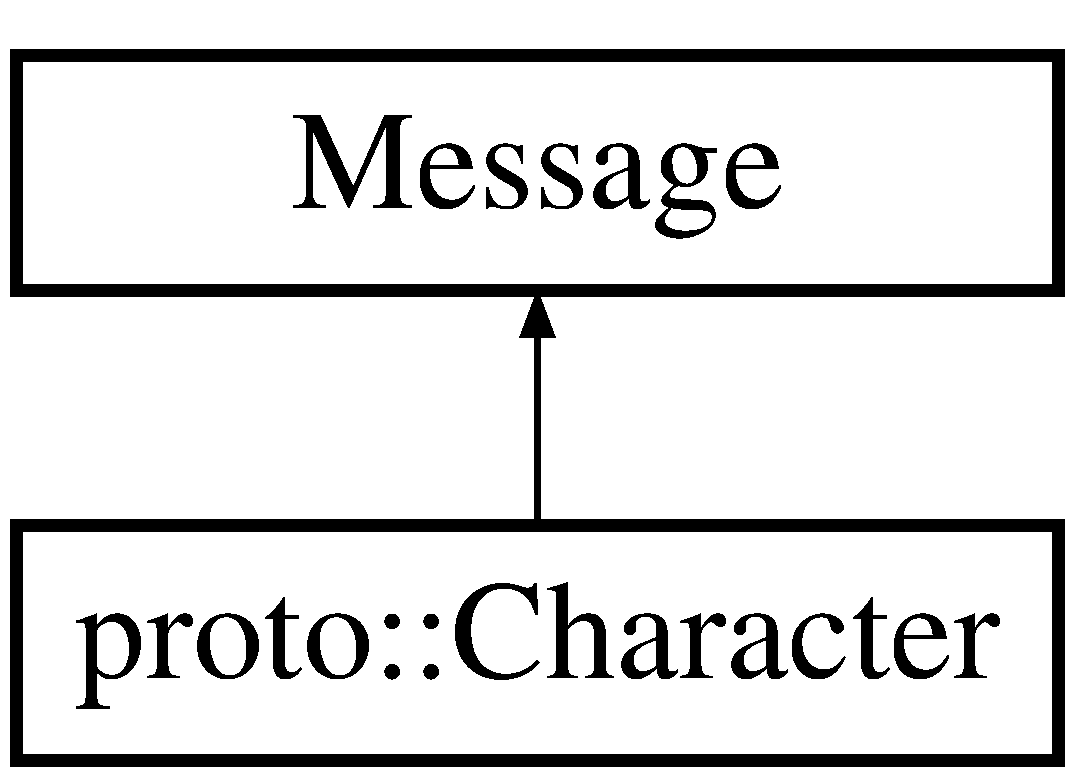
\includegraphics[height=2.000000cm]{classproto_1_1_character}
\end{center}
\end{figure}
\subsection*{Public Member Functions}
\begin{DoxyCompactItemize}
\item 
\hypertarget{classproto_1_1_character_a8f5bf8d77951e0ea45b39462a7546cdf}{}{\bfseries Character} (const \hyperlink{classproto_1_1_character}{Character} \&from)\label{classproto_1_1_character_a8f5bf8d77951e0ea45b39462a7546cdf}

\item 
\hypertarget{classproto_1_1_character_ab844330645f962034e76a4d659d83071}{}\hyperlink{classproto_1_1_character}{Character} \& {\bfseries operator=} (const \hyperlink{classproto_1_1_character}{Character} \&from)\label{classproto_1_1_character_ab844330645f962034e76a4d659d83071}

\item 
\hypertarget{classproto_1_1_character_a02f5d040d51c5a49a8dbcb164833fd50}{}const \+::google\+::protobuf\+::\+Unknown\+Field\+Set \& {\bfseries unknown\+\_\+fields} () const \label{classproto_1_1_character_a02f5d040d51c5a49a8dbcb164833fd50}

\item 
\hypertarget{classproto_1_1_character_a11846eb41c8714f5e9b4ee437de7bbca}{}inline\+::google\+::protobuf\+::\+Unknown\+Field\+Set $\ast$ {\bfseries mutable\+\_\+unknown\+\_\+fields} ()\label{classproto_1_1_character_a11846eb41c8714f5e9b4ee437de7bbca}

\item 
\hypertarget{classproto_1_1_character_ae439e522739760c54ef9d65acd53615e}{}void {\bfseries Swap} (\hyperlink{classproto_1_1_character}{Character} $\ast$other)\label{classproto_1_1_character_ae439e522739760c54ef9d65acd53615e}

\item 
\hypertarget{classproto_1_1_character_af1c934cc12cbef7ddcf73bf7197cd3db}{}\hyperlink{classproto_1_1_character}{Character} $\ast$ {\bfseries New} () const \label{classproto_1_1_character_af1c934cc12cbef7ddcf73bf7197cd3db}

\item 
\hypertarget{classproto_1_1_character_aa0496b0a8682360a40607c8f5b092875}{}void {\bfseries Copy\+From} (const \+::google\+::protobuf\+::\+Message \&from)\label{classproto_1_1_character_aa0496b0a8682360a40607c8f5b092875}

\item 
\hypertarget{classproto_1_1_character_a88ccb78cc0e4e17cb9287278cd4f6ed5}{}void {\bfseries Merge\+From} (const \+::google\+::protobuf\+::\+Message \&from)\label{classproto_1_1_character_a88ccb78cc0e4e17cb9287278cd4f6ed5}

\item 
\hypertarget{classproto_1_1_character_add0afd0f841d005acea8326ca2028d90}{}void {\bfseries Copy\+From} (const \hyperlink{classproto_1_1_character}{Character} \&from)\label{classproto_1_1_character_add0afd0f841d005acea8326ca2028d90}

\item 
\hypertarget{classproto_1_1_character_adcf70ea964c51f2608063282baeaa607}{}void {\bfseries Merge\+From} (const \hyperlink{classproto_1_1_character}{Character} \&from)\label{classproto_1_1_character_adcf70ea964c51f2608063282baeaa607}

\item 
\hypertarget{classproto_1_1_character_a42a81f720f0dc1c2e5f0ac1c03ce3251}{}void {\bfseries Clear} ()\label{classproto_1_1_character_a42a81f720f0dc1c2e5f0ac1c03ce3251}

\item 
\hypertarget{classproto_1_1_character_a99242fb29ccace1bd0e21f3a79c954fb}{}bool {\bfseries Is\+Initialized} () const \label{classproto_1_1_character_a99242fb29ccace1bd0e21f3a79c954fb}

\item 
\hypertarget{classproto_1_1_character_af8c367cdffe969e07ad8917b5a107545}{}int {\bfseries Byte\+Size} () const \label{classproto_1_1_character_af8c367cdffe969e07ad8917b5a107545}

\item 
\hypertarget{classproto_1_1_character_a9a96e8b83784508722e34b21172c7c57}{}bool {\bfseries Merge\+Partial\+From\+Coded\+Stream} (\+::google\+::protobuf\+::io\+::\+Coded\+Input\+Stream $\ast$input)\label{classproto_1_1_character_a9a96e8b83784508722e34b21172c7c57}

\item 
\hypertarget{classproto_1_1_character_a922061bd15e72f5289a3d08f0fee7002}{}void {\bfseries Serialize\+With\+Cached\+Sizes} (\+::google\+::protobuf\+::io\+::\+Coded\+Output\+Stream $\ast$output) const \label{classproto_1_1_character_a922061bd15e72f5289a3d08f0fee7002}

\item 
\hypertarget{classproto_1_1_character_a0d5473252d5df1e2093474324c05f1e3}{}\+::google\+::protobuf\+::uint8 $\ast$ {\bfseries Serialize\+With\+Cached\+Sizes\+To\+Array} (\+::google\+::protobuf\+::uint8 $\ast$output) const \label{classproto_1_1_character_a0d5473252d5df1e2093474324c05f1e3}

\item 
\hypertarget{classproto_1_1_character_a86d98fbf393ee54aa17389a9dc1bf282}{}int {\bfseries Get\+Cached\+Size} () const \label{classproto_1_1_character_a86d98fbf393ee54aa17389a9dc1bf282}

\item 
\hypertarget{classproto_1_1_character_a131cbcdb689033b8696fce65d0b890c0}{}\+::google\+::protobuf\+::\+Metadata {\bfseries Get\+Metadata} () const \label{classproto_1_1_character_a131cbcdb689033b8696fce65d0b890c0}

\end{DoxyCompactItemize}
\subsection*{Static Public Member Functions}
\begin{DoxyCompactItemize}
\item 
\hypertarget{classproto_1_1_character_af5ece1da02fa96963d539411dbc4b65f}{}static const \+::google\+::protobuf\+::\+Descriptor $\ast$ {\bfseries descriptor} ()\label{classproto_1_1_character_af5ece1da02fa96963d539411dbc4b65f}

\item 
\hypertarget{classproto_1_1_character_ad616cfe1d5e99d64cf20493e6a122b68}{}static const \hyperlink{classproto_1_1_character}{Character} \& {\bfseries default\+\_\+instance} ()\label{classproto_1_1_character_ad616cfe1d5e99d64cf20493e6a122b68}

\end{DoxyCompactItemize}
\subsection*{Friends}
\begin{DoxyCompactItemize}
\item 
\hypertarget{classproto_1_1_character_adef05d207947d9b35b104f4d265cb814}{}void {\bfseries protobuf\+\_\+\+Add\+Desc\+\_\+\+Character\+\_\+2eproto} ()\label{classproto_1_1_character_adef05d207947d9b35b104f4d265cb814}

\item 
\hypertarget{classproto_1_1_character_a60f31d05ed7be3be9b60eec3dce13a63}{}void {\bfseries protobuf\+\_\+\+Assign\+Desc\+\_\+\+Character\+\_\+2eproto} ()\label{classproto_1_1_character_a60f31d05ed7be3be9b60eec3dce13a63}

\item 
\hypertarget{classproto_1_1_character_af5b2da6541a81a0d17644f512d753edc}{}void {\bfseries protobuf\+\_\+\+Shutdown\+File\+\_\+\+Character\+\_\+2eproto} ()\label{classproto_1_1_character_af5b2da6541a81a0d17644f512d753edc}

\end{DoxyCompactItemize}


\subsection{Detailed Description}


Definition at line 40 of file Character.\+pb.\+h.



The documentation for this class was generated from the following files\+:\begin{DoxyCompactItemize}
\item 
C\+:/\+Users/\+Adewale Adekoya/\+Documents/\+Git\+Hub/\+A2/Character.\+pb.\+h\item 
C\+:/\+Users/\+Adewale Adekoya/\+Documents/\+Git\+Hub/\+A2/Character.\+pb.\+cc\end{DoxyCompactItemize}

\hypertarget{struct_skill}{}\section{Skill Struct Reference}
\label{struct_skill}\index{Skill@{Skill}}
\subsection*{Public Types}
\begin{DoxyCompactItemize}
\item 
\hypertarget{struct_skill_a460934d44040fda3fdbb9aff24cfe80f}{}enum {\bfseries Skill\+Type} \{ {\bfseries Rock}, 
{\bfseries Paper}, 
{\bfseries Scissors}
 \}\label{struct_skill_a460934d44040fda3fdbb9aff24cfe80f}

\end{DoxyCompactItemize}
\subsection*{Public Member Functions}
\begin{DoxyCompactItemize}
\item 
\hypertarget{struct_skill_a78a3b5201189083059e568bdef2606a2}{}{\bfseries Skill} (std\+::string n, \hyperlink{class_skill_type}{Skill\+Type} t)\label{struct_skill_a78a3b5201189083059e568bdef2606a2}

\end{DoxyCompactItemize}
\subsection*{Public Attributes}
\begin{DoxyCompactItemize}
\item 
\hypertarget{struct_skill_a1271744546e69259d6ac31013900c49e}{}std\+::string {\bfseries name}\label{struct_skill_a1271744546e69259d6ac31013900c49e}

\item 
\hypertarget{struct_skill_a8deae6639996545a133cf1b17d082425}{}\hyperlink{class_skill_type}{Skill\+Type} {\bfseries type}\label{struct_skill_a8deae6639996545a133cf1b17d082425}

\end{DoxyCompactItemize}


\subsection{Detailed Description}


Definition at line 7 of file S\+Kill\+Type.\+h.



The documentation for this struct was generated from the following file\+:\begin{DoxyCompactItemize}
\item 
C\+:/\+Users/\+Adewale Adekoya/\+Documents/\+Git\+Hub/\+A2/S\+Kill\+Type.\+h\end{DoxyCompactItemize}

\hypertarget{class_skill_type}{}\section{Skill\+Type Class Reference}
\label{class_skill_type}\index{Skill\+Type@{Skill\+Type}}
\subsection*{Public Member Functions}
\begin{DoxyCompactItemize}
\item 
\hypertarget{class_skill_type_a6c8a2607e7bc0137871504d681625e2b}{}{\bfseries Skill\+Type} (const Skill\+Type\+Type \&t)\label{class_skill_type_a6c8a2607e7bc0137871504d681625e2b}

\item 
\hyperlink{class_skill_type}{Skill\+Type} \hyperlink{class_skill_type_abdbb933e04dcfefbb9456c5860a6ae0a}{Get\+Skill\+Type} () const 
\item 
\hyperlink{struct_skill}{Skill} \hyperlink{class_skill_type_a34c5fa040a4bc9faa54c20f8c05969a4}{Get\+Rock\+Skill} () const 
\item 
\hyperlink{struct_skill}{Skill} \hyperlink{class_skill_type_a324e79968a5a197417aab55866ef0629}{Get\+Paper\+Skill} () const 
\item 
\hyperlink{struct_skill}{Skill} \hyperlink{class_skill_type_ae07cda8ecb9720092c435ff4eb12be3b}{Get\+Scissors\+Skill} () const 
\end{DoxyCompactItemize}
\subsection*{Static Public Member Functions}
\begin{DoxyCompactItemize}
\item 
\hypertarget{class_skill_type_ad09b4c9baf9e032726212550e00701c6}{}static \hyperlink{class_skill_type}{Skill\+Type} {\bfseries Get\+Skill\+Type} (const std\+::string \&Skill\+Type\+Name)\label{class_skill_type_ad09b4c9baf9e032726212550e00701c6}

\end{DoxyCompactItemize}
\subsection*{Protected Member Functions}
\begin{DoxyCompactItemize}
\item 
std\+::string \hyperlink{class_skill_type_a4b5a58d034a63b9b75279e22d9726947}{Get\+Skill\+Type\+Name} () const 
\end{DoxyCompactItemize}


\subsection{Member Function Documentation}
\hypertarget{class_skill_type_a324e79968a5a197417aab55866ef0629}{}\index{Skill\+Type@{Skill\+Type}!Get\+Paper\+Skill@{Get\+Paper\+Skill}}
\index{Get\+Paper\+Skill@{Get\+Paper\+Skill}!Skill\+Type@{Skill\+Type}}
\subsubsection[{Get\+Paper\+Skill() const }]{\setlength{\rightskip}{0pt plus 5cm}{\bf Skill} Skill\+Type\+::\+Get\+Paper\+Skill (
\begin{DoxyParamCaption}
{}
\end{DoxyParamCaption}
) const}\label{class_skill_type_a324e79968a5a197417aab55866ef0629}
Returns the paper skill type

\begin{DoxyReturn}{Returns}
the paper skill type to the \hyperlink{class_character}{Character} 
\end{DoxyReturn}
\hypertarget{class_skill_type_a34c5fa040a4bc9faa54c20f8c05969a4}{}\index{Skill\+Type@{Skill\+Type}!Get\+Rock\+Skill@{Get\+Rock\+Skill}}
\index{Get\+Rock\+Skill@{Get\+Rock\+Skill}!Skill\+Type@{Skill\+Type}}
\subsubsection[{Get\+Rock\+Skill() const }]{\setlength{\rightskip}{0pt plus 5cm}{\bf Skill} Skill\+Type\+::\+Get\+Rock\+Skill (
\begin{DoxyParamCaption}
{}
\end{DoxyParamCaption}
) const}\label{class_skill_type_a34c5fa040a4bc9faa54c20f8c05969a4}
Returns the Rock skill type

\begin{DoxyReturn}{Returns}
the rock skill type to the \hyperlink{class_character}{Character} 
\end{DoxyReturn}
\hypertarget{class_skill_type_ae07cda8ecb9720092c435ff4eb12be3b}{}\index{Skill\+Type@{Skill\+Type}!Get\+Scissors\+Skill@{Get\+Scissors\+Skill}}
\index{Get\+Scissors\+Skill@{Get\+Scissors\+Skill}!Skill\+Type@{Skill\+Type}}
\subsubsection[{Get\+Scissors\+Skill() const }]{\setlength{\rightskip}{0pt plus 5cm}{\bf Skill} Skill\+Type\+::\+Get\+Scissors\+Skill (
\begin{DoxyParamCaption}
{}
\end{DoxyParamCaption}
) const}\label{class_skill_type_ae07cda8ecb9720092c435ff4eb12be3b}
Returns the scissors skill type

\begin{DoxyReturn}{Returns}
the scissors skill type to the \hyperlink{class_character}{Character} 
\end{DoxyReturn}
\hypertarget{class_skill_type_abdbb933e04dcfefbb9456c5860a6ae0a}{}\index{Skill\+Type@{Skill\+Type}!Get\+Skill\+Type@{Get\+Skill\+Type}}
\index{Get\+Skill\+Type@{Get\+Skill\+Type}!Skill\+Type@{Skill\+Type}}
\subsubsection[{Get\+Skill\+Type() const }]{\setlength{\rightskip}{0pt plus 5cm}{\bf Skill\+Type} Skill\+Type\+::\+Get\+Skill\+Type (
\begin{DoxyParamCaption}
{}
\end{DoxyParamCaption}
) const}\label{class_skill_type_abdbb933e04dcfefbb9456c5860a6ae0a}
Returns the skill type

\begin{DoxyReturn}{Returns}
the name of the character 
\end{DoxyReturn}
\hypertarget{class_skill_type_a4b5a58d034a63b9b75279e22d9726947}{}\index{Skill\+Type@{Skill\+Type}!Get\+Skill\+Type\+Name@{Get\+Skill\+Type\+Name}}
\index{Get\+Skill\+Type\+Name@{Get\+Skill\+Type\+Name}!Skill\+Type@{Skill\+Type}}
\subsubsection[{Get\+Skill\+Type\+Name() const }]{\setlength{\rightskip}{0pt plus 5cm}std\+::string Skill\+Type\+::\+Get\+Skill\+Type\+Name (
\begin{DoxyParamCaption}
{}
\end{DoxyParamCaption}
) const\hspace{0.3cm}{\ttfamily [protected]}}\label{class_skill_type_a4b5a58d034a63b9b75279e22d9726947}
\hyperlink{struct_skill}{Skill} Type name. 

The documentation for this class was generated from the following files\+:\begin{DoxyCompactItemize}
\item 
C\+:/\+Users/\+Adewale Adekoya/\+Documents/\+Git\+Hub/\+A2/S\+Kill\+Type.\+h\item 
C\+:/\+Users/\+Adewale Adekoya/\+Documents/\+Git\+Hub/\+A2/Skill\+Type.\+cpp\end{DoxyCompactItemize}

\hypertarget{structproto_1_1_static_descriptor_initializer___character__2eproto}{}\section{proto\+:\+:Static\+Descriptor\+Initializer\+\_\+\+Character\+\_\+2eproto Struct Reference}
\label{structproto_1_1_static_descriptor_initializer___character__2eproto}\index{proto\+::\+Static\+Descriptor\+Initializer\+\_\+\+Character\+\_\+2eproto@{proto\+::\+Static\+Descriptor\+Initializer\+\_\+\+Character\+\_\+2eproto}}


The documentation for this struct was generated from the following file\+:\begin{DoxyCompactItemize}
\item 
C\+:/\+Users/\+Adewale Adekoya/\+Documents/\+Git\+Hub/\+A2/Character.\+pb.\+cc\end{DoxyCompactItemize}

\hypertarget{struct_weapon}{}\section{Weapon Struct Reference}
\label{struct_weapon}\index{Weapon@{Weapon}}
\subsection*{Public Member Functions}
\begin{DoxyCompactItemize}
\item 
\hypertarget{struct_weapon_a3066227b3eb4195b1e28b7c2b0c660f6}{}{\bfseries Weapon} (std\+::string n)\label{struct_weapon_a3066227b3eb4195b1e28b7c2b0c660f6}

\end{DoxyCompactItemize}
\subsection*{Public Attributes}
\begin{DoxyCompactItemize}
\item 
\hypertarget{struct_weapon_a8bc12bf0ac8e3cdea9c8657ccb6217b5}{}std\+::string {\bfseries name}\label{struct_weapon_a8bc12bf0ac8e3cdea9c8657ccb6217b5}

\end{DoxyCompactItemize}


The documentation for this struct was generated from the following file\+:\begin{DoxyCompactItemize}
\item 
C\+:/\+Users/\+Adewale Adekoya/\+Documents/\+Git\+Hub/\+A2/S\+Kill\+Type.\+h\end{DoxyCompactItemize}

%--- End generated contents ---

% Index
\backmatter
\newpage
\phantomsection
\clearemptydoublepage
\addcontentsline{toc}{chapter}{Index}
\printindex

\end{document}
